\documentclass[11pt]{report}

\usepackage[utf8]{inputenc} % Required for inputting international characters
\usepackage[T1]{fontenc} % Output font encoding for international characters
\usepackage[a4paper, total={7in, 10in}]{geometry}
\usepackage{mathpazo} % Palatino font
\usepackage{graphicx}
\usepackage{sectsty}
\usepackage{lipsum} 
\usepackage{pgfgantt}
\usepackage{afterpage}
\usepackage{wrapfig}
% \usepackage{indentfirst}
\usepackage{float}
\usepackage{framed}
\usepackage[pagestyles]{titlesec}
\renewcommand\bibname{References}
% \titleformat{\chapter}{\bfseries\centering}{}{0pt}{\Huge}
\titleformat{\chapter}[display]
  {\normalfont\huge\bfseries}
  {}
  {0pt}
  {\filcenter\Huge\scshape}
\titlespacing*{\chapter}{0pt}{40pt}{40pt}
\titleformat*{\section}{\Large\bfseries}
\titleformat*{\subsection}{\large\bfseries}

\renewcommand*\footnoterule{}
% \newpagestyle{mystyle}
% {\sethead[\thepage][][\chaptertitle]{}{}{\thepage}}
% \pagestyle{mystyle}
\pagestyle{plain}
\setlength{\FrameSep}{10pt}
\setlength{\FrameRule}{1pt}
\newcommand{\HRule}{\rule{\linewidth}{1pt}\bigskip\par}
% \allsectionsfont{\centering}

\begin{document}
\begin{center}
\textbf{\LARGE\textsc{Department of Computer Science and Engineering}}\bigskip\\
\textbf{\Large{VIII Semester Project}}\bigskip\\
\textbf{\huge\textsc{Monthly Progress Report - II}}\bigskip\\
\end{center}
\begin{framed}
\noindent \large{Batch No. }\hspace{64pt}\textbf{\large{35}}\medskip\\
\large{Title of the project: }\hspace{17pt}\textbf{\large\textsc{Image Regeneration using Generative Models}}\medskip\\
\noindent\begin{tabular}{@{}l@{\hspace{31pt}}l r }
\large{Team members: }  & {\large \textbf{Abhijith C.}}       & \large \textbf{1MV14CS004} \\
                        & {\large \textbf{Raghava G. Dhanya}} & \large \textbf{1MV14CS077} \\
                        & {\large \textbf{Shashank S.}}       & \large \textbf{1MV14CS131}
\end{tabular}\\[15pt]  
\noindent \large{Name of the Guide: }\hspace{12pt}\textbf{\large{Sushila Shidnal}}\medskip\\
\noindent \large{Duration: }\hspace{65pt}\textbf{\large{From March Week 1 to April Week 1}}\medskip\\
\HRule
\noindent \textbf{\Large{Details Of Work Carried Out:}}\bigskip\\
\indent On week 3 of march we were able to implement a CapsNet based binary classifier based on Geoffrey Hinton \textit{et al.}\footnotemark[1]. On week 4 of march we tried to create a CapsNet based Generator, We encountered a problem, we were not able to inverse the dynamic routing in CapsNet to reverse the architecture for Generator. \par
\begin{wrapfigure}{l}{0.3\textwidth}
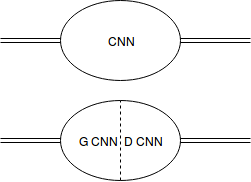
\includegraphics[width=.3\textwidth]{CapsGAN.png}
\caption{A normal capsule vs our proposed capsule}
\label{fig:capsgan}
\end{wrapfigure} 
After considering multiple alternatives, We came up with a new architecture for Generator using CapsNet. This architecture is based on using the knowledge of dynamic routing from the Discriminator to perform dynamic routing in Generator. In a general CapsNet each capsule contains convolutional network, We can see these as a small Convolutional Neural Network(CNN). In a DCGAN there are two DCNN working in adversarial fashion. We propose an architecture for Capsule generator in figure \ref{fig:capsgan} where each of the capsule will contain a small GAN having both generator and discriminator in it. Generator will be inactive while discriminator is learning, when generator is learning it remembers the dynamic routing from the discriminator and uses it to find the higher level capsule to which it needs to route the generated data. The higher level capsule generator uses this as their noise input to generate the Image.\par
The next step in the process was to figure out the mathematics for the training of the CapsuleGAN. We have come up with few methods and we will be implementing these methods and the proposed architecture and compare the results the state of the art GAN's in the following weeks.
\end{framed}
\footnotetext[1]{Sara Sabour, Nicholas Frosst, and Geoffrey E Hinton. Dynamic routing between capsules. In I. Guyon, U. V. Luxburg, S. Bengio, H. Wallach, R. Fergus, S. Vishwanathan, and R. Garnett, editors, Advances in Neural Information Processing Systems 30, pages 3856–3866. Curran Associates, Inc., 2017.}
\afterpage{
\begin{framed}
\noindent \textbf{\Large{Time-line:}}\\[10pt]

\includegraphics[width=1.1\textwidth]{timeline.png}\\[10pt] 
\noindent\HRule
\vspace{50px}
\centering
\textbf{Head of the Department}
\vspace{50px}
\flushleft\textbf{Project Guide}\hfill\textbf{Project Coordinator}
\end{framed}
}
\end{document}